% !Mode:: "TeX:UTF-8"
% !TEX root = ..\thesis.tex
\newcommand{\jobunit}[1]{*+[F]{\makebox[1.5em]{$#1$}}}
\newcommand{\process}[1]{*++=[o][F]{\makebox[2em]{$#1$}}}
\newcounter{algor}%\newcounter{exam}
\theoremheaderfont{\heiti}
\newtheorem{algori}[algor]{算法}%\newtheorem{exam}[exam]{示例}
\newcounter{local}
\chapter{算法设计}
上一章构建了$2$个多品种产品调度的数学模型,需要对其检验,而这些模型求解是NP--Hard问题,需要设计相应算法来求解。在求解模型前,需要对订单处理时间计算,该问题也需通过算法设计求解。模型的具体求解算法可以分为构造型和改进型,前者从没有调度的情况开始,按一定分派规则逐渐安排作业,直至生成一个较好的调度;后者则是在前者的基础上,调整已有调度以改善目标。

\section{分派规则}
前文已提到的EDD规则和FCFS规则是常见的调度分派规则,在具体调度作业的时候,通常会先根据分派规则进行安排,所以分派规则便是作业安排的初始策略,然后再局部调整调度方案以进一步优化。一个周详的规则可能得到最优调度的初始解,显然简化了局部调整过程,然而极可能会需要巨大的思考空间和时间(比如枚举)。同样,过于直觉的规则将会增大后续调整的难度,所以制定分派规则时要作权衡。
\subsection{基本规则}
\begin{asparaenum}
\item EDD(最早交货期)
\suspend{asparaenum}

EDD规则从工期角度出发,将作业按照交货时刻的先后进行排序,并按这个顺序进行生产处理。对于并行机环境,一旦某处理单元空闲,就可以即刻安排队列中的首个作业任务。这个规则适用于安排目标和工期相关的调度任务。
\resume{asparaenum}
\item WSPT(加权最短处理时间)
\suspend{asparaenum}

WSPT规则是SPT(最短处理时间)规则的一般化,从作业的处理时间出发,对以完工时刻为目标的调度任务较为合适。这个规则将处理作业按照$w_j/p_j$值非增的顺序排列,处理时间较长的作业被安排在较后的位置,从一定程度上减少了排队等待时间,并且可以证明WSPT规则对$1\mid \mid \sum w_jC_j$的调度是最优的\cite{pinedo},然而在$Pm \mid \mid \sum w_jC_j$ 环境下并不一定是最优。

\resume{asparaenum}
\item MS(最小松弛)
\end{asparaenum}

MS规则通过描述作业的紧迫程度来进行作业调度,与前两者最大的区别在于,这个规则是动态的,即和系统时间$t$相关。作业根据$\max \{d_j - p_j - t , 0\}$的值非减的顺序排列,显然较为紧迫的作业会被安排在前面,并且不同的系统时间会影响排列的顺序,呈现动态的调度。该规则适用于安排目标和工期相关的调度任务。
\subsection{复合规则}
复合分派规则是综合了许多基本规则的一个表达式,各基本规则都有其各自的比例参数,用来确定这个规则对符合规则影响程度的比例,没有固定的形式,接下来举一例:ATC(明显滞后成本)规则。

ATC规则综合了WSPT规则和MS规则,每当有空闲处理单元时,所有待调度作业按\eqref{equ:orderindexexample}计算其排序指数,选出具有最大指数值的作业进行处理。
\begin{equation}
I_j(t) = \frac{wt_j}{p_j}\exp\left(-\frac{\max\{d_j - p_j - t, 0\}}{K\bar p}\right) \label{equ:orderindexexample}
\end{equation}
式中:

\begin{tabular}{ll}
$K$ & 规则比例参数\\
$\bar p$ &剩余作业平均处理时间
\end{tabular}

可以看出当$K \to \infty$时,$I_j(t) \to w_j/p_j$,此时ATC规则便转化为WSPT规则。当$K \to 0$时,若作业$j$将产生延期,即$\max(d_j - p_j -t , 0 ) = 0$,那么ATC规则也转化为WSPT规则,若作业不会产生延期,由于$d_j - p_j - t$的影响超过$w_j/p_j$,规则ATC将转化为MS规则。ATC规则可以较容易地应用到$Pm\mid\mid \sum w_jT_j$问题。

\section{基本模型}
基本模型由目标函数\eqref{equ:objmain}和约束条件\eqref{equ:basicst1} -- (\ref{equ:basicst7})组成,其最优调度的求解包括初始可行解与解的改进,分别在构造型和改进型算法中详述。
\subsection{构造算法}
构造算法的主要内容是确定分派规则,虽然不能保证得到最优调度,但却有着很高的执行性,便于计划安排。基本模型的目标函数主要成分是为加权时延迟间总和,采用ATC规则能得到较优调度\footnote{准确来说,ATC规则较为适用于$1\mid\mid \sum w_jT_j$ 问题,对于$Pm\mid\mid \sum w_jT_j$也能得到质量很高的解,虽然这个规则运用于基本模型所涉及的问题效果不一定如这两个确切的问题,但足够作为后续改进的初始调度},关键在于比例参数的选取,相关的方法也有很多,例如回归分析、机器学习等。本课题将该规则得到的调度作为改进算法的初始解,所以不需要在该参数上过多深究,可以采用$K = 2$作为推荐值\cite{bilge2007tabu}。

针对基本模型的实际情况,调度中的作业为各订单,并用整合处理时间作为各订单的处理时间,这样可以不考虑切换准备时间。此外,后续的改进算法要用到构造算法的相关信息,需要记录被调度的订单序列。为了方便描述这个算法以及后续算法,需要扩充符号说明如下:

\begin{tabular}{ll}
$J$ & 待调度订单集合\\
$L$ & 已调度的订单记录序列,其集合记为$\overline{L}$\\
$L_j$ & 订单记录序列的第$j$项作业,$(j = 1,2,...,n)$\\
$a_l$ & 流水线运行状态,处理订单时$a_l = 1$,否则$a_l = 0$,$(l = 1,2,...,m)$\\
$t_l$ & 流水线$l$的预计正在处理订单的完成时刻,$(l = 1,2,...,m)$\\
$G(S)$& 调度$S$的目标函数\\
$H(S_l)$ & 流水线$l$的调度目标函数\\
$h(j)$ & 订单$j$的目标函数\\
$S^{(0)}$ & 目前为止的最佳调度\\
$S^{(c)}$& 相邻调度,即候选调度\\
$\overline{S^{(c)}}$& 邻域调度集合\\
$|S^{(c)}|$& 邻域容量,即相邻调度的数量\\
$TL$ & 禁忌列表\\
$NL$ &禁忌列表长度\\
$A$ & 特赦解\\
$NR$ &交替次数
\end{tabular}

\begin{algori}
基本模型ATC规则调度构造算法\label{alg:basicconstruct}

\begin{asparaenum}
\renewcommand{\labelenumi}{\bf Step\theenumi~}
\item 初始化。$J = N, \overline{L} = \varnothing$, $t_l = 0, \overline{S_l} = \varnothing, a_l=0, (l = 1,2,...,m)$,根据和\refa{alg:processtime}计算各订单处理时间$p'_j = g(j, n_j)$,进一步得到整合订单处理时间$p_j = p'_j + s_j, (j = 1,2,...,n)$,置系统时间$t = 0$;
\item 若存在$a_l = 0$,记$l^* = \displaystyle\min_{a_l = 0}\{l\}$,执行\Step{3},否则执行\Step{4};
\item 根据\eqref{equ:orderindexexample},选取预备调度订单$j^*$,使得$I_{j^*}(t) = \displaystyle\max_{j\in J}\{I_j(t)\}$,将订单$j^*$安排入流水线$l^*$进行处理,记入调度$S_{l^*}$,$\overline{S_{l^*}}=\overline{S_{l^*}}\bigcup \{j^*\}$, $J = J -\{j^*\}$,记录调度订单序列$\overline{L} = \overline{L} \bigcup \{j^*\}$,更新流水线预计空闲时刻$t_{l^*} = t + p_{j^*}$,修改流水线状态$a_{l^*} = 1$。若$J = \varnothing$,所有订单调度完毕,终止算法,否则执行\Step{2};
\item 记$lt$使得 $t_{lt} = \displaystyle\min_{1\le l\le m}\{t_l\}$,修改流水线状态$a_{lt} = 0$,并更新系统时间$t = t_{lt}$,执行\Step{2}。
\end{asparaenum}
\end{algori}

\subsection{改进算法}
构造算法得到的初始解需要进行改进,为了尽可能得到较优解,需要采用一些启发式(元启发式)算法,区域搜索是一类较为有效并且操作简便的算法,其主要的两个步骤是邻域的定义与移动选择。对于多机环境,一般采用分阶段的交替算法。此外,本文提出的一种虚拟序列算法克服了交替算法的一些劣势。

\subsubsection{邻域定义}
为了后面相关算法的描述,需要先定义邻域。考虑第一种情况,某机器上有共$4$项作业(标记为$1,2,3,4$),其初始调度$S^{(1)}$安排如\reff{fig:4example}所示,
\begin{figure}[h]
\begin{equation*}
\xymatrix{
\jobunit{1} \ar[r] & \jobunit{2} \ar[r] &\jobunit{3} \ar[r] &\jobunit{4}
}
\end{equation*}
\caption{$4$项作业的初始调度$S^{(1)}$示例\label{fig:4example}}
\end{figure}
箭头方向为作业处理的顺序方向。交换$S^{(1)}$中相邻两项作业的顺序,可以得到一个新的调度$S^{(2)}$,显然此例中$S^{(2)}$有如\reff{fig:3neighbors}所示的$3$种可能。这三个不同的调度构成了调度$S^{(1)}$的邻域,而确定其中的一个作为$S^{(2)}$便是一次移动选择。至此,机器内的邻域及移动定义完毕。

\begin{figure}[h]
\centering
\vspace{1.5em}
\subfloat[交换$1,2$]{
\xymatrix{
\jobunit{2} \ar[r] & \jobunit{1} \ar[r] &\jobunit{3} \ar[r] &\jobunit{4}
}}\\
\subfloat[交换$2,3$]{
\xymatrix{
\jobunit{1} \ar[r] & \jobunit{3} \ar[r] &\jobunit{2} \ar[r] &\jobunit{4}
}}\\
\subfloat[交换$3,4$]{
\xymatrix{
\jobunit{1} \ar[r] & \jobunit{2} \ar[r] &\jobunit{4} \ar[r] &\jobunit{3}
}}
\caption{$S^{(1)}$的$3$个相邻调度\label{fig:3neighbors}}
\end{figure}

接下来考虑另一种情况,在多机环境下,机器间的作业移动。如果只是简单的从某个机器上挑选某个作业移动到另一个机器的某个位置,这样定义的邻域容量约为$2\sum\sum n_i\times n_j$,($n_i,n_j$为机器$i,j$上的作业数量),不但会和前一种情况的邻域重叠,其过大的容量对搜索来说也是不合理的。所以机器间的邻域及移动要按照具体情况来设计定义。

\subsubsection{交替算法}
通常并行机环境的改进算法分为两个阶段,机器内部的作业序列改变和机器间的作业改派,这两个过程交替进行\cite{史烨2011},然而这个方法十分费时,但简化内部改进则又影响解的质量。本节将提出一种新的邻域结构,巧妙地避免了前面的问题。
一般来说,由ATC规则所得到的该模型的初始解是较优解,甚至可能是最优解,如果需要对其改进,需要从两个方面来考虑。一个是流水线内部订单序列的调整,另一个是流水线间的订单调整,这两种调整涉及两种元启发式算法,需要交替使用。
\begin{asparaenum}
\item 内部调整
\suspend{asparaenum}

流水线内部调整是$1\mid\mid \sum w_jT_j$问题的一种扩展,可以简单运用ATC规则达到较好解,不同与前面的并行机环境,单机环境下,对流水线$l$使用ATC调度作业的具体算法如下。

\begin{algori}
基本模型ATC规则调度改进算法\label{alg:atcinner}
\begin{asparaenum}
\renewcommand{\labelenumi}{\bf Step\theenumi~}
\item 初始化。$J = \overline{S_l}$,根据和\refa{alg:processtime}计算各订单处理时间$p'_{l_k} = g({l_k}, |S_l|)$,进一步得到整合订单处理时间$p_{l_k} = p'_{l_k} + s_{l_k}(k = 1,2,...,|S_l|)$,置系统时间$t = 0$,重置$\overline{S_l} = \varnothing$;
\item 根据\eqref{equ:orderindexexample},选取预备调度订单$l_k^*$,使得$I_{l_k^*}(t) = \displaystyle\max_{l_k\in J}\{I_{l_k}(t)\}$,将订单$l_k^*$进行安排处理,$J = J -\{l_k^*\}$,将该订单排入该流水线的调度$\overline{S_l} = \overline{S_l}\bigcup \{l_k^*\} $。若$J = \varnothing$,该流水线上的订单调度完毕,终止算法,否则执行\Step{3};
\item 更新系统时间$t = t + p_{l_k^*}$,执行\Step{2}。
\end{asparaenum}
\end{algori}

也可以对流水线$l$采用区域搜索的方法改进进行,该流水线上的调度邻域和前面的机器内部邻域类似,作业的序列就相当于流水线上订单的序列,初始调度$S_l^{(1)}$由\refa{alg:basicconstruct}得到,如\reff{fig:initlschedule}所示。
\begin{figure}[h]
\begin{equation*}
\xymatrix{
\jobunit{l_1} \ar[r] & \jobunit{l_2} \ar[r]& \jobunit{l_3} \ar[r]&\cdots\ar[r] &\jobunit{l_{|S_l|}}
}
\end{equation*}
\caption{流水线的初始调度$S_l^{(1)}$\label{fig:initlschedule}}
\end{figure}
这样一来,对于每条流水线的内部调整改进,每次生成的调度都有$|S_l|-1$个相邻的调度可供移动,并以相邻订单对$(l_j, l_k)$来表示解的一次移动。若每次都向着目标值改进最大的方向移动,则可能陷入局部最优解。可以采用一些机制避免此类情况发生,不同的机制原理便产生了不同的元启发式搜索算法。根据基本模型的特征,本文将采用改进过的禁忌所搜算法,它的机理是在移动选择时,为了不落入局部最优的循环而有意识地避开,需要设定禁忌列表$TL$及其长度$NL$,通常禁忌列表满时候,采用FIFO规则将项目出栈。基本模型下,流水线$l$的内部调整禁忌搜索总结如下。
\begin{algori}
内部调整禁忌搜索算法
\begin{asparaenum}
\renewcommand{\labelenumi}{\bf Step\theenumi~}
\item 初始化。设定迭代次数$N_I$,清空禁忌列表$TL$,设定列表长度$NL$,将构造算法所得的调度作为初始调度,并记为当前最优调度,$S^{(0)} = S^{(1)} = S_l$,并置$k = 1$;
\item 从$S^{(k)}$所有不在禁忌列表中的相邻移动$(l_j,l_k)$中,所得调度具有最小函数值的移动,记为$(l_j^*, l_k^*)$,所得调度记为$S^*$,并置$S^{(k+1)} = S^*$;
\item 将相邻移动$(l_j^*, l_k^*)$入栈禁忌列表,若列表容量已满,则按FIFO规则出栈最早的相邻移动;
\item 若$G(S^*) < G(S^{(0)})$,置$S^{(0)} = S^*$;
\item 置$k = k + 1$,若$k\le N_I$,执行\Step{2},否则终止算法。
\end{asparaenum}
\label{alg:intertabu}
\end{algori}

\resume{asparaenum}
\item 之间调整
\suspend{asparaenum}

前面的部分说明了流水线内的订单调度改进,然而即使所有流水线都按照其相应的最优调度进行生产处理,从全局来看,这样的调度安排未必就是最优,这主要是由流水线使用不均衡引起的,这种不均衡性只能通过流水线之间的订单交换或重派来改变。将流水线$a$上的订单$a_j$重新安排在流水线$b$上的操作称为\textbf{订单重派},两流水线间的订单交换可以看作是这两条流水线互相订单重派。因此,全局调度关于流水线之间的相邻移动可以定义为某订单重派。

为提高流水线均衡性,订单重派策略为:从具有最大目标值$H(S_l)$的流水线中选取具有最大函数值$h(l_k)$的作业,将其重派至具有最小目标值的流水线上调度末端,因此需要定义流水线$l$的函数贡献值与各订单的函数贡献值,根据\eqref{equ:objmain}可得两贡献值值的定义:
\begin{align}
H(S_l) &= \lambda_t\sum_{k=1}^{|S_l|} wt_{l_k}T_{l_k} + \lambda_c\sum_{k=1}^{|S_l|}wc_{l_k}C_{l_k}\label{equ:linefunct}\\
h(l_k) &= \lambda_t wt_{l_k}T_{l_k} + \lambda_c wc_{l_k}C_{l_k}
\label{equ:itemfunct}
\end{align}
这个策略可以用一个确定性的算法得到。
\begin{algori}
流水线之间订单重派算法\label{alg:between}
\begin{asparaenum}
\renewcommand{\labelenumi}{\bf Step\theenumi~}
\item 计算各流水线的$H(S_l)$值,选出具有最大值与最小值的流水线,记为$l^+, l^-$;
\item 计算流水线$l^+$的调度$S_{l^+}$中具有最大$h(l_k)$值的订单$l^+_{k^*}$,并将其添入流水线$l^-$的调度$S_{l^-}$末端。
\end{asparaenum}
\end{algori}

\resume{asparaenum}
\item 交替改进
\end{asparaenum} 

产生初始调度后,各流水线上的调度需要通过内部调整以局部改进,然后通过流水线之间的订单重派对现有解进行扰动,此时被添派订单的流水线则需要再调整一次以合理安排新添入的订单。如此交替操作便是这个算法的基本策略。
\begin{algori}
基本模型交替算法\label{alg:inturnbasic}
\begin{asparaenum}
\renewcommand{\labelenumi}{\bf Step\theenumi~}
\item 运用\refa{alg:basicconstruct}建立流水线全局调度初始解;
\item 运用\refa{alg:intertabu}(或\refa{alg:atcinner})改进所有流水线的初始调度,设定交替次数$NR$,置$k = 1$;
\item 运用\refa{alg:between}重派订单,并将被派单的流水线记为$l^*$;
\item 运用\refa{alg:intertabu}(或\refa{alg:atcinner})对流水线$l^*$进行调整改进;
\item 置$k = k+1$,若$k\le NR$,执行\Step{3},否则终止算法。
\end{asparaenum}
\end{algori}

\subsubsection{虚拟序列算法}
尽管\refa{alg:inturnbasic}得到了质量较高的调度,然而由于其交替结构的特点,导致这个算法需要花较长的时间却比一定能达到预期的改进。为了使解的改进调整更为全局性,同时减少计算时间,本节将从另一个角度分析问题,提出一个更为合理的虚拟序列算法。

所谓虚拟序列,即将所有流水线上的调度看作一个整体,所有订单都在这个序列上,其排列顺序由初始解的生成规则决定,也就是在调度安排时的记录序列$L$,并按先后顺序记该序列上的订单为$L_j, (j = 1,2,...,n)$。显而易见的是,任意流水线上两订单的先后顺序和它们在虚拟序列中的顺序是一样的。

虚拟序列上只有所有订单的先后信息,其订单的一种排序称为一种\textbf{虚拟调度}。虚拟调度的邻域设计和流水线内部调度类似,一次移动改变对于虚拟序列本身来说,就是该序列中两相邻的订单处理顺序交换,而体现在各流水线则要分为以下两种情况。
\begin{asparaenum}
\item 相邻订单$L_j, L_k$安排在同一条流水线$l$上进行处理
\suspend{asparaenum}

该情况下,现有调度的一种可行移动就是这两个相邻订单的交换。
\resume{asparaenum}
\item 相邻订单$L_j, L_k$分别安排在不同流水线$l, l'$上进行处理
\end{asparaenum}

该情况下,现有调度关于该两相邻订单的交换可以有$3$种移动:
\begin{inparaenum}
\renewcommand{\theenumi}{\protect\setcounter{local}{171 + \the\value{enumi}}\protect\ding{\value{local}}}
\renewcommand{\labelenumi}{\theenumi}
\item 将这两个订单的位置互换,即$L_j$安排在流水线$l'$上订单$L_k$的原有位置,订单$L_k$亦然\label{item:situation1};
\item 将订单$L_j$重派到流水线$l'$上,其位置与$L_k$相邻,顺序和此次移到后的虚拟序列中两订单的顺序一致;
\item 将订单$L_k$重派到流水线$l$上,其位置与$L_j$相邻,顺序和此次移到后的虚拟序列中两订单的顺序一致。
\end{inparaenum}

后面两种情况在作移动时,不需要将订单交换对入栈禁忌列表,因为若再作一步该交换对的移动,不会回到之前的状态,而情况\ref{item:situation1}则只对两订单交换位置的移动禁忌。若虚拟序列中相邻订单对$(L_j, L_k)$交换作为一次移动,其算法如下。
\begin{algori}
虚拟序列邻域生成\label{alg:vituralneighbor}
\begin{asparaenum}
\renewcommand{\labelenumi}{\bf Step\theenumi~}
\item 输入预交换订单对$(L_j, L_k)$,记当前调度为$S^-$,若$L_j, L_k$当前均安排在同一流水线的调度中,则执行\Step{2},否则执行\Step{3};
\item 交换订单对顺序,得到新的调度为$S^+$型;
\item 将订单$L_j$重派入流水线$l'$,得到调度为$S^{a+}$型,或将订单$L_k$重派入流水线$l$得到调度为$S^{b+}$型,或将订单$L_j, L_k$交换位置,得到调度为$S^+$型;
\item 更新虚拟序列中这两个订单的位置为$(L_k, L_j)$。
\end{asparaenum}
\end{algori}
可以看出,一个调度的邻域容量不是一个定值,会随着调度结构的改变而改变。

\begin{algori}
虚拟序列禁忌搜索算法
\begin{asparaenum}
\renewcommand{\labelenumi}{\bf Step\theenumi~}
\item 运用\refa{alg:basicconstruct}建立流水线全局调度初始解,得到虚拟序列$L$及其初始调度$S^{(0)}$,并将其作为目前最优调度。设定禁忌搜索迭代次数$N_I$,设定列表长度$NL$,并置特赦调度$A = S^{(0)}$;
\item 置$S^{(1)} = S_{(0)}$,清空禁忌列表$TL$,置$k = 1$;
\item 根据\refa{alg:vituralneighbor}中的邻域生成算法,检查禁忌列表中的订单对,若它们别安排在不同的流水线,则只对其交换位置的移动禁忌;若移动后的调度为特赦调度,一样认定为可行移动。计算$S^{(k)}$中所有可行移动组成的邻域,选取它们中具有最小函数值调度的移动,记该订单对为$(L_j^*, L_k^*)$,所得调度记为$S^*$,并置$S^{(k+1)} = S^*$;
\item 若相邻移动所得调度属于$S^+$型,则将$(L_j^*, L_k^*)$入栈禁忌列表,若列表容量已满,则按FIFO规则出栈最早的相邻移动;
\item 若$G(S^*) < G(S^{(0)})$,置$S^{(0)} = S^*$;
\item 置$k = k + 1$,若$k\le N_I$,执行\Step{3},否则终止算法,$S^{(0)}$为最终所得调度。
\end{asparaenum}
\end{algori}

\section{陆续模型}
陆续模型由目标函数\eqref{equ:insertobj}和约束条件\eqref{equ:insertst1} -- (\ref{equ:insertst13})组成,与基本模型类似,其最优调度的求解包括初始可行解与解的改进,分别在构造型和改进型算法中详述。
\subsection{构造算法}
基本模型的构造算法基于ATC分派规则,因为其主要目标是加权延迟时间和的变形,而陆续模型是基本模型的更为一般的形式,主要是进一步考虑了切换准备时间\footnote{基本模型中也考虑切换准备时间,只是由于该模型的特性,可以将其与订单处理时间合并成整合处理时间,以简化模型求解。而陆续模型需要分开考虑这两个时间}和订单进入系统时刻。可以继续使用ATC 规则,然而本节将要使用其推广形式中的一种:ATCS\footnote{ATCS规则是专门为$1\mid s_j\mid\sum w_jT_j$问题所设计的} (考虑准备时间的明显滞后成本)。

ATCS 规则是WSPT 规则、MS 规则和SST (最小切换准备时间)规则的复合规则,每当有空闲处理单元时,所有待调度作业按\eqref{equ:orderindexexample2}计算其排序指数,选出具有最大指数值的作业进行处理。
\begin{equation}
I_j(t) = \frac{w_j}{p_j}\exp\left(-\frac{\max\{d_j - p_j - t, 0\}}{K_1\bar p} - \frac{s_j}{K_2 \bar s}\right) \label{equ:orderindexexample2}
\end{equation}
式中:

\begin{tabular}{ll}
$K_1$ & 与工期相关的规则比例参数\\
$K_2$ & 与切换准备时间的规则比例参数\\
$\bar p$ &剩余作业平均处理时间\\
$\bar s$ & 剩余作业平均切换准备时间
\end{tabular}

为了确定比例参数$K_1, K_2$,需要定义一些辅助变量,以作为比例参数的函数输入量。工期紧迫度可以定义为:
\[
\tau = 1 - \frac{\sum d_j}{nC_{\max}}
\]
$\tau\to 1$表明工期紧迫,反之亦然。工期范围因子可以定义为:
\[
R = \frac{d_{\max} - d_{\min}}{C_{\max}}
\]
以及切换准备时间重要性因子:
\[
\eta = \frac{\sum s_j}{\sum p_j}
\]

$K_1, K_2$在确定之前,需要对作业制造时间$C_{\max}$进行估计,可以简单估计如下:
\[
\hat C_{\max} = \frac{1}{m}\sum_{j = 1}^n p_j + \frac{1}{m}\sum_{j=1}^n s_j
\]
然后可以根据下式确定$K_1$:
\begin{subnumcases}{K_1 = }
4.5 + R & $R\le 0.5 \notag$ \\
6 - 2R & $R > 0.5$ \notag
\end{subnumcases}
以及$K_2$:
\[
K_2 = \frac{\tau}{2\sqrt{\eta}}
\]

同基本模型算法类似,运用ATCS 规则时,调度中的作业为各订单,当有流水线空闲的时候,即可根据\eqref{equ:orderindexexample2}安排订单进入相应流水线进行处理,与基本模型不同,陆续模型在安排订单的时候,需要预估流水线的闲置时间。
\begin{algori}
陆续模型的ATCS 规则调度构造算法\label{alg:continuecconstruct}

\begin{asparaenum}
\renewcommand{\labelenumi}{\bf Step\theenumi~}
\item 初始化。$J = N, \overline{L} = \varnothing$, $t_l = 0, \overline{S_l} = \varnothing, a_l=0, C_{l_0} = 0, (l = 1,2,...,m)\footnote{$C_{l_0}$是人为定义的边界量,便于后续算法的初始情况}$,根据和\refa{alg:processtime}计算各订单处理时间$p_j = g(j, n_j), (j = 1,2,...,n)$,置系统时间$t = 0$;
\item 若存在$a_l = 0$,记$l^* = \displaystyle\min_{a_l = 0}\{l\}$,执行\Step{3},否则执行\Step{5};
\item 根据\eqref{equ:orderindexexample2},选取预备调度订单$j^*$,使得$I_{j^*}(t) = \displaystyle\max_{j\in J}\{I_j(t)\}$,将订单$j^*$安排入流水线$l^*$进行处理,记入调度$S_{l^*}$,$\overline{S_{l^*}}=\overline{S_{l^*}}\bigcup \{j^*\}$, $J = J -\{j^*\}$,记录调度订单序列$\overline{L} = \overline{L} \bigcup \{j^*\}$;
\item 置$k = |S_{l^*}|$,对于流水线$l^*$,将订单$j^*$标记为$l^*_k$,预估订单$l^*_k$开始处理前的流水线闲置时间$f_{j^*} = f_{l^*_k} = \max\{r_{l^*_k} - s_{l^*_k}- C_{l^*_{k-1}}, 0\}$,更新流水线预计空闲时刻$t_{l^*} = t + p_{j^*} + s_{j^*} + f_{j^*}$,修改流水线状态$a_{l^*} = 1$。若$J = \varnothing$,所有订单调度完毕,终止算法,否则执行\Step{2};
\item 记$lt$使得 $t_{lt} = \displaystyle\min_{1\le l\le m}\{t_l\}$,修改流水线状态$a_{lt} = 0$,并更新系统时间$t = t_{lt}$,执行\Step{2}。
\end{asparaenum}
\end{algori}

\subsection{改进算法}
与基本模型的改进算法类似,陆续模型的改进算法可以通过两阶段的交替算法,也可以直接使用虚拟序列算法。
\subsubsection{交替算法}
交替算法分为内部调整和之间调整,由于陆续模型的特点,其算法和基本模型的略有不同,下面进行分述。
\begin{asparaenum}
\item 内部调整
\suspend{asparaenum}

各流水线的作业内部调整可以简单实用ATCS 规则,但该规则最为合适的问题环境与本模型有一些差别,为了得到较好的调度效果,可以采用禁忌搜索来调整调度。其算法基本和\refa{alg:intertabu}一致,其区别仅在目标函数上,将其替换即可。

\resume{asparaenum}
\item 之间调整
\suspend{asparaenum}

流水线之间的调整在于订单重派,而订单重派则的依据是流水线和订单对目标函数的贡献值,需要根据\eqref{equ:insertobj}来重新定义这两个贡献值函数:
\begin{align}
H(S_l) &= \lambda_1\frac{\sum_{k=1}^{|S_l|}\sqrt{w_{l_k}^2L_{l_k}^2}}{Ru_l} + \lambda_2 \exp\left(-\frac{Rb}{\sigma}\right)\sum_{k=1}^{|S_l|}wc_{l_k}C_{l_k}\label{equ:lineinsertfunct}\\
h(l_k) &= \lambda_1\frac{\sqrt{w_{l_k}^2L_{l_k}^2}}{Ru_l} + \lambda_2 \exp\left(-\frac{Rb}{\sigma}\right)wc_{l_k}C_{l_k}
\label{equ:iteminsertfunct}
\end{align}

然后应用\refa{alg:between}可以得到陆续模型的流水线之间的调度调整。
\resume{asparaenum}
\item 交替算法
\end{asparaenum}

在得到初始调度之后,首先要对每条流水线进行内部调整,然后结合流水线的内部和之间调整,并交替这两个步骤。
\begin{algori}
陆续模型交替算法\label{alg:inturncontinue}
\begin{asparaenum}
\renewcommand{\labelenumi}{\bf Step\theenumi~}
\item 运用\refa{alg:continuecconstruct}建立流水线全局调度初始解;
\item 运用\refa{alg:intertabu}改进所有流水线的初始调度,设定交替次数$NR$,置$k = 1$;
\item 运用\refa{alg:between}重派订单,并将被派单的流水线记为$l^*$;
\item 运用\refa{alg:intertabu}对流水线$l^*$进行调整改进;
\item 置$k = k+1$,若$k\le NR$,执行\Step{3},否则终止算法。
\end{asparaenum}
\end{algori}

\subsubsection{虚拟序列算法}
基本模型中已经阐述并应用了虚拟序列,并设计了相应的算法,虚拟序列同样也适用于陆续模型。
对于虚拟序列,可以像基本模型一样,直接使用禁忌搜索,不过由于虚拟序列长度要远大于任一流水线的调度序列长度,跳出局部最优需要的步骤可能会很多,可以考虑将其结合变动邻域搜索(VNS)来直接切换邻域结构,当然这么做也可能会跳出含有最优解的邻域分支。
\begin{algori}
虚拟序列VN - Tabu 搜索算法
\begin{asparaenum}
\renewcommand{\labelenumi}{\bf Step\theenumi~}
\item 运用\refa{alg:continuecconstruct}建立流水线全局调度初始解,得到虚拟序列$L$及其初始调度$S^{(0)}$,并将其作为目前最优调度,将其邻域集合$\overline{S^{(c)}}$中的调度按函数值的非减排列,记为$S_{[1]},S_{[2]},...,S_{[|S^{(c)}|]}$,置$i = 1$。设定禁忌搜索迭代次数$N_I$,设定列表长度$NL$,并置特赦调度$A = S^{(0)}$;
\item 若$i \le |S^{(c)}|$,置$S^{(1)} = S_{[i]}$,清空禁忌列表$TL$,置$k = 1$,否则终止算法;
\item 根据\refa{alg:vituralneighbor}中的邻域生成算法,检查禁忌列表中的订单对,若它们别安排在不同的流水线,则只对其交换位置的移动禁忌;若移动后的调度为特赦调度,一样认定为可行移动。计算$S^{(k)}$中所有可行移动组成的邻域,选取它们中具有最小函数值调度的移动,记该订单对为$(L_j^*, L_k^*)$,所得调度记为$S^*$,并置$S^{(k+1)} = S^*$;
\item 若相邻移动所得调度属于$S^+$型,则将$(L_j^*, L_k^*)$入栈禁忌列表,若列表容量已满,则按FIFO规则出栈最早的相邻移动;
\item 若$G(S^*) < G(S^{(0)})$,置$S^{(0)} = S^*$;
\item 置$k = k + 1$,若连续$10$次采用没有更新$S^{(0)}$,则置$i = i+1$,执行\Step{2},否则若$k\le N_I$,执行\Step{3},否则终止算法,$S^{(0)}$为最终所得调度。
\end{asparaenum}
\end{algori}
\section{订单处理时间计算}
前一章提到,各订单的处理时间与被处理的流水线无关,只与其所含作业数量相关,因此可将订单的处理时间看作是关于订单本身及其所含作业数量的函数,记为$p_j = g(j,n_j)$,其中$n_j$为订单$j$所含的作业数量。此外,仍需要补充符号说明如下:\\[3pt]
\begin{supertabular}{ll}
$n_j$ & 订单$j$所含的作业数量\\
$k$ & 作业标记,$k = 1,2,...,n_j$\\
$m_j$ & 订单$j$的处理单元数量\\
$i$ & 订单$j$的处理单元标记,$i = 1,2,...,m_j$\\
$q_{k,i}$ & 作业$k$在处理单元$i$上的处理时间\\
$c_{k,i}$ &作业$k$的在处理单元$i$上的完成时刻\\
$c_{j,\max}$ & 订单$j$中所有作业的制造期,即$\max(c_k)$\\
\end{supertabular}\\[3pt]
其中不同作业在同处理单元上的处理时间相同,可以简记为$q_i$。

由于订单和子单仅有作业数量的差别,故考虑订单的情况即可推广到子单。由于,产品体积小,可以假设处理单元间的缓冲空间足够用。订单在某条流水线上的作业可以看作是流水车间环境,没有换线时间,所以该问题可以记为:$Fm\mid \mid C_{\max}$,显而易见的是 $c_{j,\max} = c_{n_j,m_j}$。该问题的数学模型如下:
\begin{gather}
\min c_{n_j, m_j}\\[-2pt]
\text{s.t.}\notag
\end{gather}
\begin{numcases}{}
c_{1,1} = q_{1,1}\label{equ:processtime1}\\
c_{1,i} = \sum_{i=1}^{m_j} q_{1,i}\label{equ:processtime2}\\
c_{k,1} = c_{k-1,1} + q_{k,1} & $k = 2,3,...,n_j$\\
c_{k,i} = \max\{c_{k-1,i} ,c_{k,i-1}\} &$k = 2,3,...,n_j, i = 2,3,...,m_j$\\
q_{k,i}  = q_i & $k = 1,2,...,n_j, i = 1,2,...,m_j$
\end{numcases}

该问题可以用有向图来表示,其关键路径即为所求解的计算历程。如\ref{fig:directedgraph}所示,每个节点内表示作业的处理时间,横向表示作业处理顺序,纵向表示不同的处理单元,由左上角开始,按照有向弧的方向进入节点,计算出右下节点的时间即为订单处理时间。
其中,\eqref{equ:processtime1}和(\ref{equ:processtime2})可以化简得到这个等式:$c_{k,1} = k\cdot q_1,(k = 1,2,...,n)$,便于下面算法的初始化。
\begin{figure}[h]
\begin{equation*}
\xymatrix{
\process{q_{1,1}} \ar[r] \ar[d] & \process{q_{1,2}} \ar[d] \ar[r] & \cdots\ar[r] & \process{q_{1,m_j}} \ar[d]\\
\process{q_{2,1}} \ar[r]\ar[d] & \process{q_{2,2}} \ar[d]\ar[r] & \cdots \ar[r] \ar[d]& \process{q_{2,m_j}} \ar[d] \\
\vdots\ar[d] & \vdots \ar[d]\ar[r] & \process{q_{k,i}}\ar[r]\ar[d] &\vdots \ar[d]\\
\process{q_{n_j,1}} \ar[r] & \process{q_{n_j,2}} \ar[r] & \cdots\ar[r] & \process{q_{n_j,m_j}}
}
\end{equation*}
\caption{订单的作业处理有向图\label{fig:directedgraph}}
\end{figure}

也可以从生产节拍的角度来得到订单的装配处理时间。由于订单中的作业是相同的,所以生产节拍为订单的瓶颈工序,即$\displaystyle tt_j = \max_{1\le i\le m_j}\{q_i\}$,也就是说,除了首项作业的处理时间为各工序处理时间总和,其余作业皆按节拍完成,那么订单$j$的装配处理时间为:
\[
p_j = \sum_{i = 1}^{m_j}q_i + (n_j - 1)tt_j
\]



\section{小结}

tikz 作图
\begin{figure}[h]
\centering
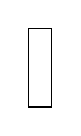
\begin{tikzpicture}
\draw (0,0) rectangle (0.3,1.00);
\end{tikzpicture}
\end{figure}